\documentclass[fullscreen=true, bookmarks=true, hyperref={pdfencoding=unicode}]{beamer}
\usepackage[utf8]{inputenc}                                % Кодировка
\usepackage[english,russian]{babel}                        % Переносы
\usepackage{xcolor}                                        % Работа с цветом
\usepackage{amsmath,amssymb,amsfonts}                      % Символы АМО
\usepackage{graphicx}                                      % Графика
\usepackage[labelsep=period]{caption}                      % Разделитель в подписях к рисункам и таблицам
\usepackage{hhline}                                        % Для верстки линий в таблицах
\usepackage{tikz}                                          % Для простых рисунков в документе
\usepackage{fancybox}                                      % Пакет для отрисовки рамок
\usepackage{verbatim}                                      % Для вставки кода в презентацию
\usepackage{animate}                                       % Для вставки видео в презентацию
\usepackage{xmpmulti}                                      % Для вставки gif в презентацию
\usepackage{multirow}

\usetikzlibrary{arrows, snakes, backgrounds}                 % Для отрисовки стрелок
\usetikzlibrary{positioning, fit, arrows.meta, shapes, calc}
% used to avoid putting the same thing several times...
% Command \empt{var1}{var2}
\newcommand{\empt}[2]{$#1^{\langle #2 \rangle}$}

\graphicspath{{images/}}                                   % Путь до рисунков
\setbeamertemplate{caption}[numbered]                      % Включение нумерации рисунков

\definecolor{links}{HTML}{2A1B81}                          % blue for url links
\hypersetup{colorlinks,linkcolor=,urlcolor=links}          % nothing for others

\usetheme{Boadilla}
\usecolortheme{whale}

\usepackage{minted}

% \setbeameroption{show notes}
\setbeameroption{hide notes}
% \setbeameroption{show only notes}

\title{Lecture 9. Recurrent Neural Networks}
\author{Alex Avdyushenko}
\institute{Kazakh-British Technical University}
\date{November 5, 2022}
\titlegraphic{
\includegraphics[keepaspectratio,width=0.4\textwidth]{logo_kbtu.png}}

\begin{document}
%\unitlength=2mm

% выводим заглавие
\begin{frame}
\transdissolve[duration=0.2]
\titlepage
\end{frame}

\note{Good afternoon, dear students. Today we move on to a discussion of recurrent neural networks. This is a very interesting approach, also similar to human information processing. 

Imagine yourself reading a book, left to right, top to bottom, sentence by sentence. It turns out that neural networks now can also do something like this.}

\begin{frame}
  \frametitle{Five-minutes block}
  \pause
  \begin{itemize}
     \item Write down several names of neural network optimization methods
     \item Describe a couple of regularization methods for training neural networks
     \item Draw (or write down) how the skip-connection block works
  \end{itemize}

\end{frame}

\note{Great, let's start with traditional five-minutes questions. Please, write answers or send photos with them directly to me in private messages here in Teams or may be in Telegram, but choose only one option please :)}

\begin{frame}
\frametitle{Disadvantages of Convolutional Neural Networks}
   \framesubtitle{Or why we need recurrent ones :)}
   \begin{itemize}
     \pause
     \item the input is only fixed-dimensional vectors (e.g. 28$\times$28 images)
     \pause
     \item the output is also a fixed dimension (for example, probabilities of 1000 classes)
     \pause
     \item fixed number of computational steps (i.e. network architecture)
   \end{itemize}

   \pause
   \vspace{1cm}
   \href{http://karpathy.github.io/2015/05/21/rnn-effectiveness/}{A. Karpathy. The Unreasonable Effectiveness of Recurrent Neural Networks}
   \begin{center}
     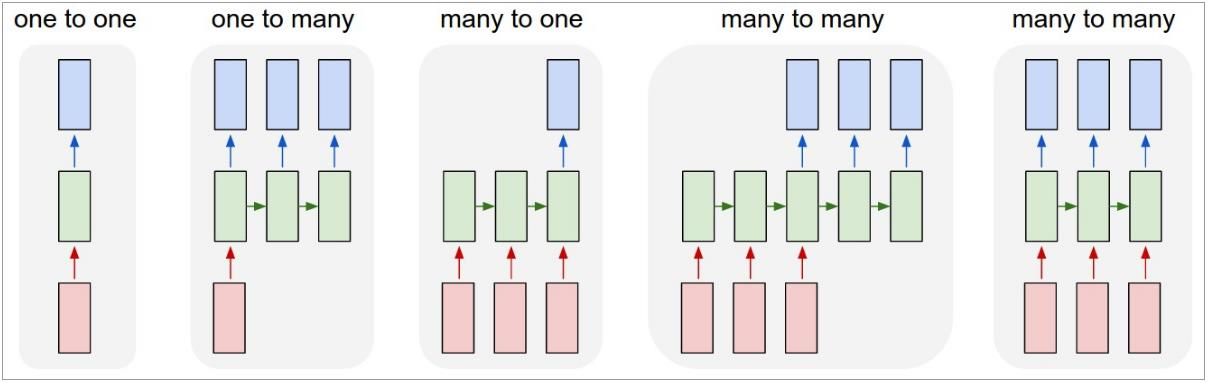
\includegraphics[keepaspectratio,
                      width=0.6\paperwidth]{rnn_architectures.jpg}
   \end{center}

\end{frame}

\note{So, how to eliminate all these disadvantages? There are several different architectures. Let's look at them one by one.}

\begin{frame}
\frametitle{Architectures of Recurrent Networks}
   \begin{center}
       \begin{tabular}{cc}
         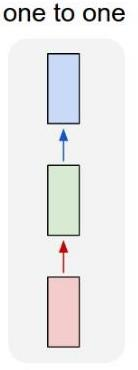
\includegraphics[keepaspectratio,
                          width=0.2\paperwidth]{one-to-one.jpg} &
         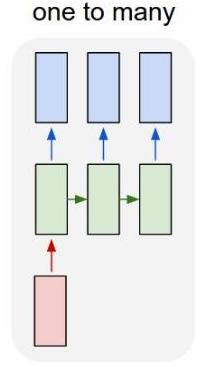
\includegraphics[keepaspectratio,
                          width=0.3\paperwidth]{one-to-many.jpg} \\
         Vanilla Neural Networks & Image Captioning \\
          & image $\to$ (sequence of words)
       \end{tabular}
   \end{center}
\end{frame}


\begin{frame}
  \begin{tabular}{cc}
    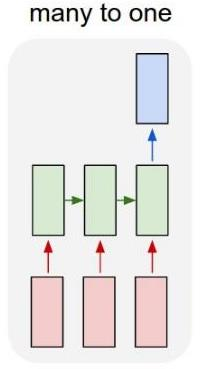
\includegraphics[keepaspectratio,
                     width=0.25\paperwidth]{many-to-one.jpg} &
    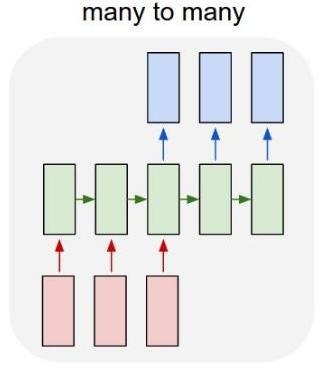
\includegraphics[keepaspectratio,
                     width=0.4\paperwidth]{many-to-many.jpg} \\
    Sentiment Classification & Machine Translation \\
     (sequence of words) $\to$ sentiment & (seq of words) $\to$ (seq of words)
  \end{tabular}
\end{frame}


\begin{frame}
  \begin{center}
    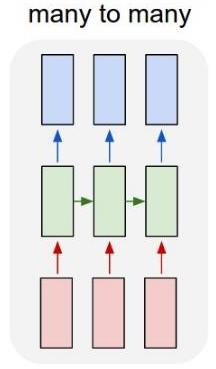
\includegraphics[keepaspectratio,
                     width=0.3\paperwidth]{many-to-many-2.jpg}

    Video Classification

    (on frame level)
  \end{center}
\end{frame}


\begin{frame}
  \frametitle{Sequential Processing of Fixed Input}
  \begin{center}
    \animategraphics[loop,width=0.28\paperwidth,autoplay]{8}{house_read-}{0}{191}
  \end{center}

  \noindent\rule{8cm}{0.4pt}

  {\small \href{https://arxiv.org/abs/1412.7755}{J. Ba, V. Mnih, K. Kavukcuoglu. Multiple Object Recognition with Visual Attention}}

\end{frame}

\note{The interesting fact is, that different recurrent architectures have also been successfully applied to problem with fixed input, such as object recognition for example.}


\begin{frame}
  \frametitle{Sequential Generation of Fixed Output}
  \begin{center}
    \animategraphics[loop,width=0.5\paperwidth,autoplay]{8}{house_generate-}{0}{37}
  \end{center}

  \noindent\rule{8cm}{0.4pt}

  {\small \href{https://arxiv.org/abs/1502.04623}{K. Gregor, I. Danihelka, A. Graves, D. J. Rezende, D. Wierstra. DRAW: A Recurrent Neural Network For Image Generation}}

\end{frame}

\note{And even image generation too!}

\begin{frame}[t]
  \frametitle{Recurrent Neural Network scheme}
  \begin{center}
    \begin{picture}(150, 125)
      \multiput(0,0)(35, 0){6}{
        \put(-25, 45){\vector(1, 0){25}}
      }
      \multiput(0,0)(35, 0){5}{
        \put(5, 5){\vector(0, 1){25}}
        \put(5, 60){\vector(0, 1){25}}
      }
      \multiput(0,0)(35, 0){5}{
        \put(0, 0){
          \put(0, 30){\framebox(10, 30){}}
        }
      }
      \put(-2, 0){\makebox{$x_{t-2}$}}
      \put(33, 0){\makebox{$x_{t-1}$}}
      \put(71, 0){\makebox{$x_{t}$}}
      \put(103, 0){\makebox{$x_{t+1}$}}
      \put(138, 0){\makebox{$x_{t+2}$}}
      \put(70, 42){\makebox{$h_{t}$}}
      \put(-2, 89){\makebox{$y_{t-2}$}}
      \put(33, 89){\makebox{$y_{t-1}$}}
      \put(71, 89){\makebox{$y_{t}$}}
      \put(103, 89){\makebox{$y_{t+1}$}}
      \put(138, 89){\makebox{$y_{t+2}$}}
    \end{picture}
  \end{center}

\end{frame}

\note{Ok, so what is inside the recurrent network, how this model works? You have some iteration proccess, where on each step one and the same function changes the hidden vector of model.}

\begin{frame}[t]
  \frametitle{Recurrent Neural Network}

  We process the sequence of vectors $x$ with {\bf one and the same} function with parameters:

   $$ h_t = f_W(h_{t-1}, x_t)$$

   $f_W$ is a function parameterized by $W$

   $x_t$ — next input vector

   $h_t$ — hidden state
   \pause
   \begin{block}{Question}
   What function can we take as $f_W$?
   \end{block}
\end{frame}

\note{Which function, one of the simplest, you know from machine learning?}

\begin{frame}[t]
  \frametitle{Vanilla Recurrent Neural Network}

  $$ h_t = f_W(h_{t-1}, x_t)$$

  As a function $f_W$ we set a linear transformation with a non-linear component-wise "sigmoid":

  \begin{align*}
    h_t &= \tanh ({\color{red}W_{hh}} h_{t-1} + {\color{red}W_{xh}} x_t) \\
    y_t &= {\color{red}W_{hy}} h_t
  \end{align*}
\end{frame}


\begin{frame}
\frametitle{Character level model example}

    The entire four-letter dictionary: $[h, e, l, o]$ and word ``hello'' as train:

    \begin{center}
      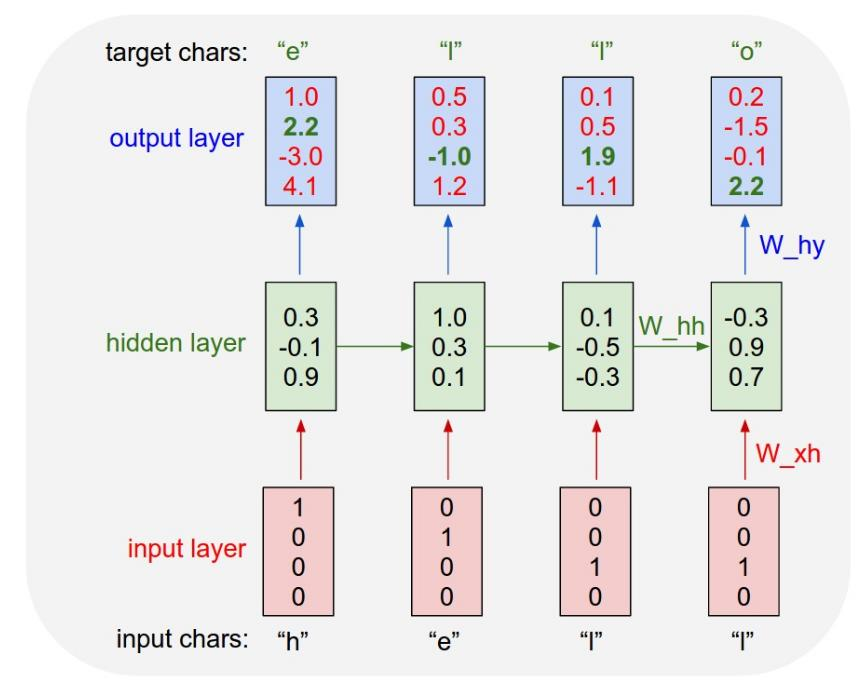
\includegraphics[keepaspectratio,
                       width=0.6\paperwidth]{rnn_char_level_example.jpg}
    \end{center}

    {\bf Softmax} is also applied to the values of the output layer to obtain the loss function
\end{frame}


\begin{frame}
  \frametitle{Demo}

  \href{https://gist.github.com/karpathy/d4dee566867f8291f086}{{\bf numpy} implementation by Karpathy}

  \vspace{1cm}
  \href{https://github.com/avalur/ml-course-kbtu/tree/main/week09_rnn/rnn_demo.ipynb}{Let's get to grips with the code in jupyter notebook!}
\end{frame}


\begin{frame}
  \frametitle{How does it work?}

  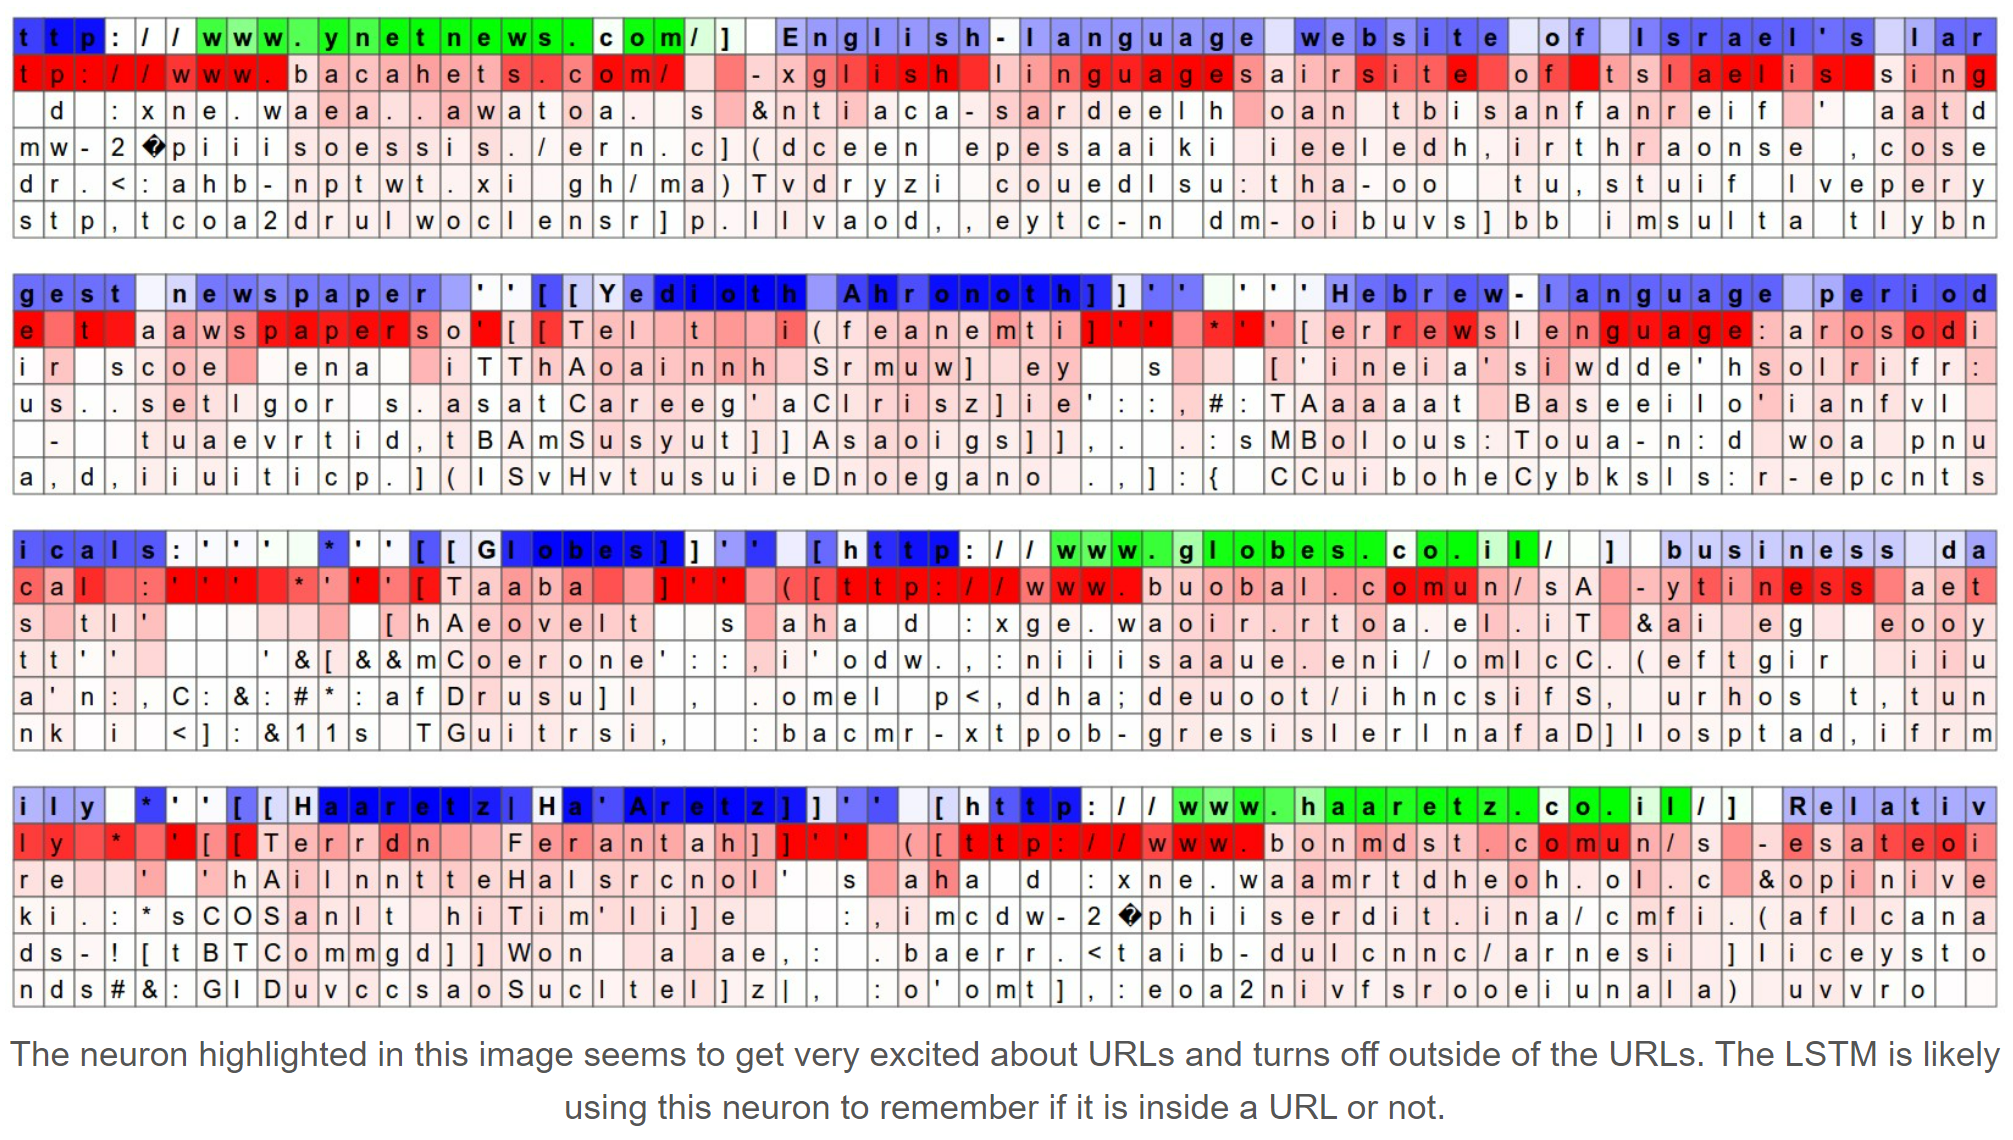
\includegraphics[keepaspectratio,
                   width=.85\paperwidth]{url_neuron.png}

\end{frame}

\note{In his work on the analysis of recurrent networks, Andrej Karpathy tried to understand the mechanisms of this model.}

\begin{frame}
  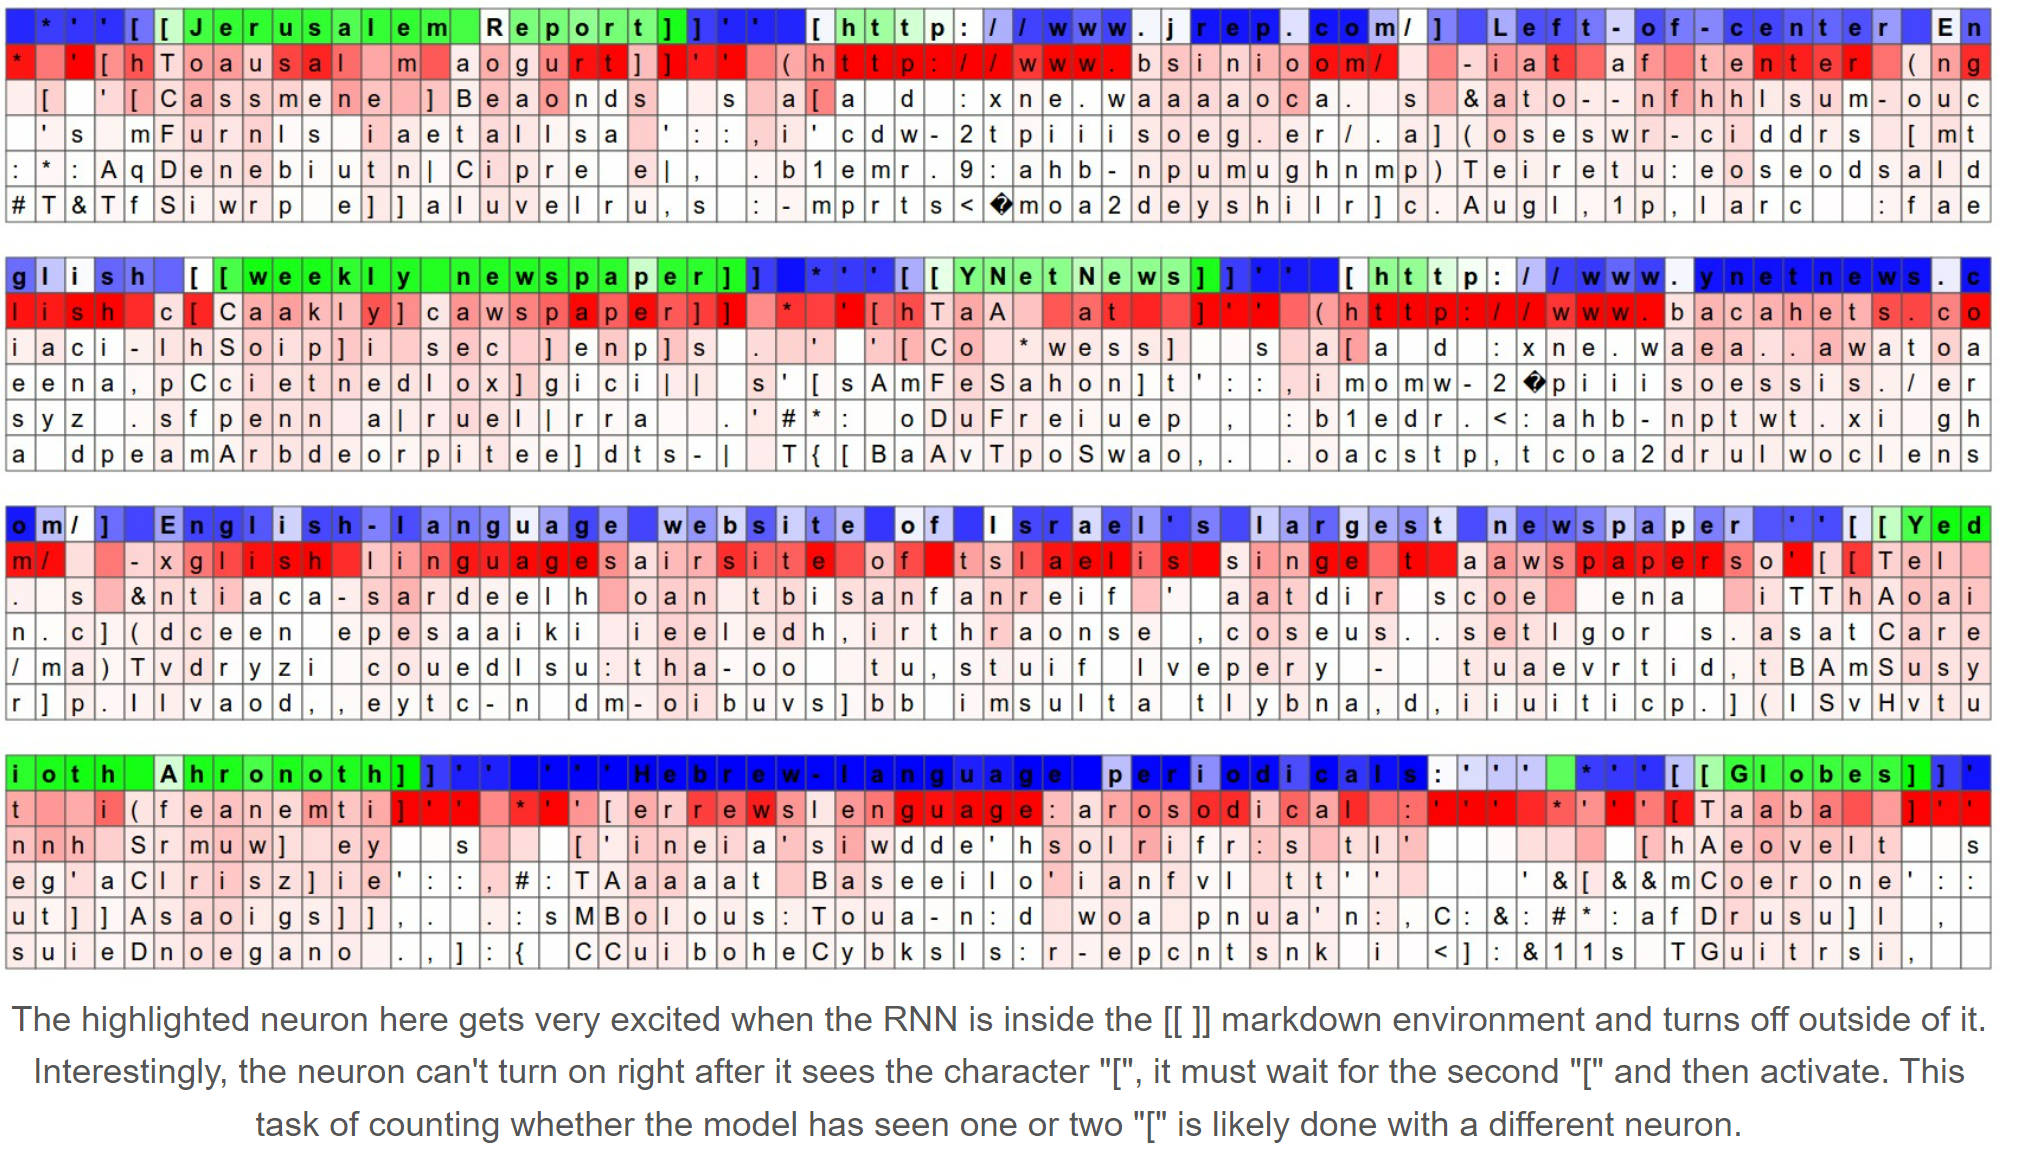
\includegraphics[keepaspectratio,
                   width=.85\paperwidth]{bracket_neuron.png}

\end{frame}


\begin{frame}
  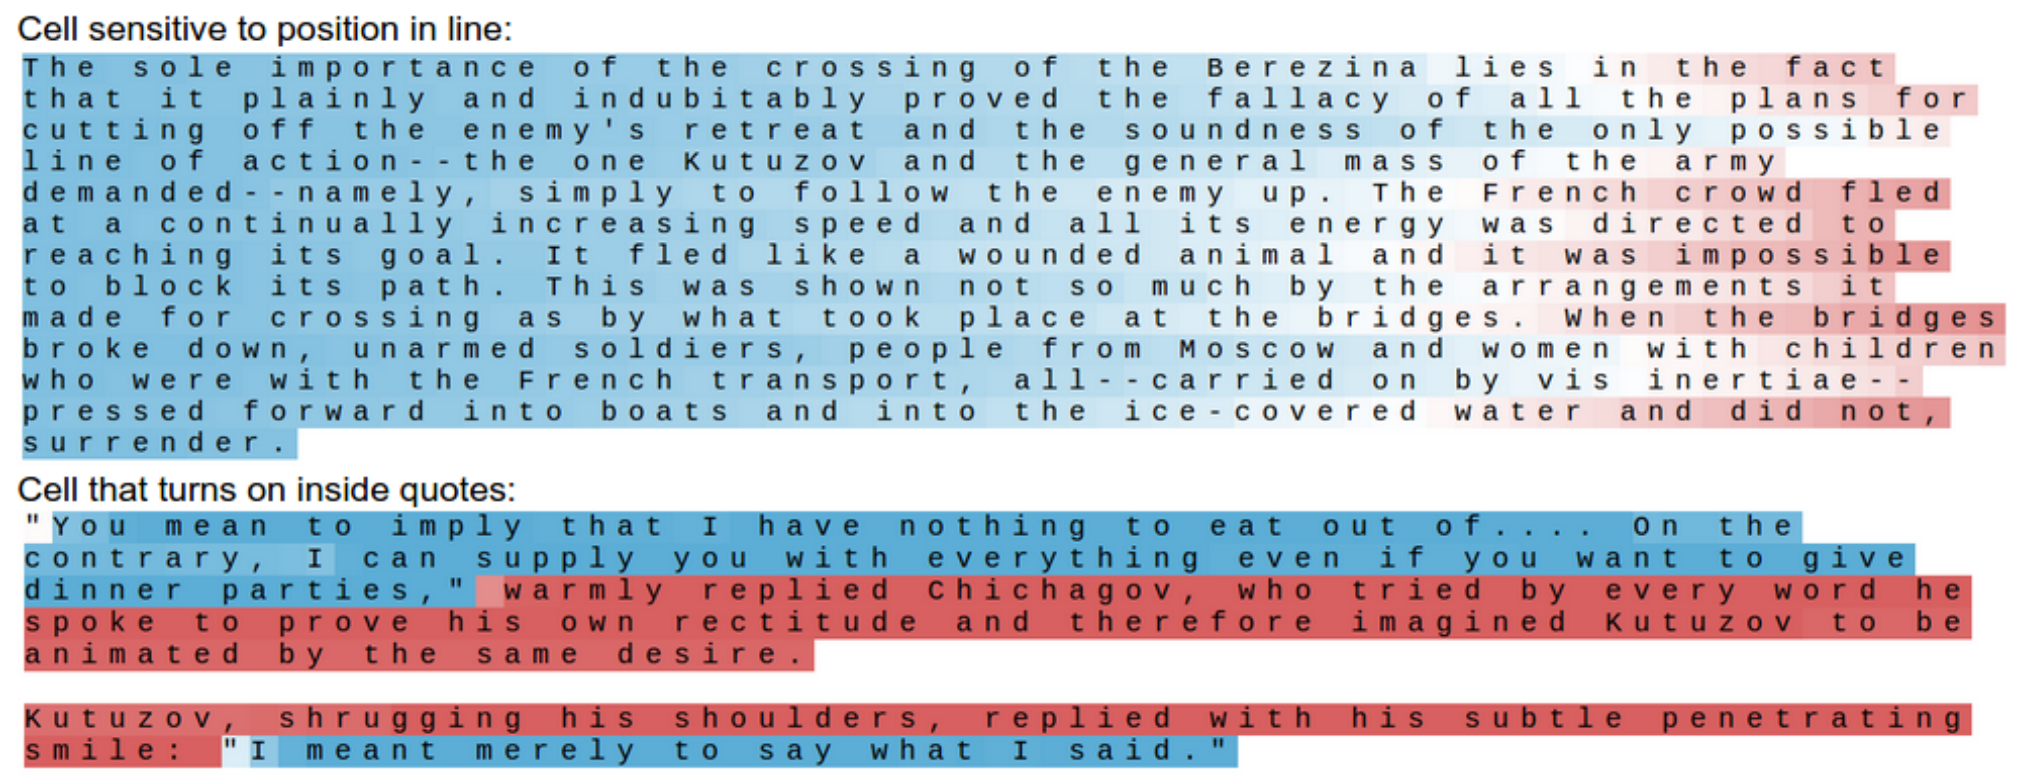
\includegraphics[keepaspectratio,
                   width=.85\paperwidth]{cell_endline.png}
\end{frame}

\note{You see, he discovered really interesting facts about RNN mechanics and showed it well with specific examples.}

\begin{frame}
  \frametitle{Deep recurrent networks}
  \begin{columns}
      \begin{column}{.4\paperwidth}
        $\quad h_t^\ell = \tanh W^\ell \left(\begin{array}{c}
         h_t^{\ell-1} \\ h_{t-1}^{\ell}
        \end{array}\right)$

        $\quad h \in \mathbb{R}^n, \quad\quad W^\ell [n \times 2n]$
      \end{column}
      \begin{column}{.4\paperwidth}
        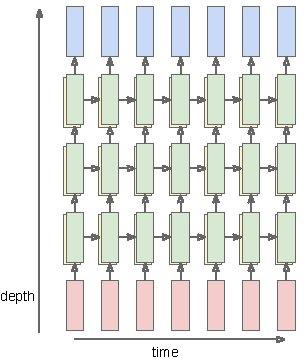
\includegraphics[keepaspectratio,
                         width=0.4\paperwidth]{rnn_depth.jpg}
      \end{column}
  \end{columns}
  \pause
  \begin{block}{Question}
  What is the main problem with vanilla RNN?
  \end{block}
\end{frame}

\note{Let's go on and talk about deep RNN with several layers. So you simply add new layers in depth.

It is difficult for RNN to remember a long context.}

\begin{frame}[t]
  \frametitle{Long short-term memory (LSTM)}

  \begin{align*}
     &W^\ell [4n\times 2n] \\
    \left(\begin{array}{c}
    i \\ f \\ o \\ c_t^\prime
    \end{array}\right) &=
    \left(\begin{array}{c}
    \text{sigm} \\ \text{sigm} \\ \text{sigm} \\ \tanh
    \end{array}\right)
    W^\ell
    \left(\begin{array}{c}
    h_t^{\ell-1} \\ h_{t-1}^{\ell}
    \end{array}\right) \\
    &\begin{array}{l}
    c_t^\ell = f \odot c_{t-1}^\ell + i \odot c_t^\prime \\
    h_t^\ell = o \odot \tanh(c_t^\ell)
    \end{array}
  \end{align*}
  \center $\odot$ — component-wise product
\end{frame}

\note{LSTM modules come to the rescue! Now you have three gates and new vector in the model — cell state.}

\begin{frame}
\frametitle{LSTM: Motivation and Schema}

   The network should remember the context for a long time. Which context? Network learns itself.
   To do this, the vector $c_t$ is introduced, which is the state vector of the network at the moment $t$.

  \vspace{1cm}
  \begin{tabular}{ll}
    $c_t^\prime = \tanh(W_{xc}x_t + W_{hc}h_{t-1} + b_{c^\prime})$ & candidate cell state \\
    $i_t = \sigma(W_{xi}x_t + W_{hi}h_{t-1} + b_{i})$ & input gate \\
    $f_t = \sigma(W_{xf}x_t + W_{hf}h_{t-1} + b_{f})$ & forget gate \\
    $o_t = \sigma(W_{xo}x_t + W_{ho}h_{t-1} + b_{o})$ & output gate \\
     & \\
    $c_t = f_t \odot c_{t-1} + i_t \odot c_t^\prime$ & cell state \\
    $h_t = o_t \odot \tanh(c_t)$ & block output
  \end{tabular}
\end{frame}


\begin{frame}
  \begin{center}
  \begin{tikzpicture}[
    % GLOBAL CFG
    font=\sf \scriptsize,
    >=LaTeX,
    % Styles
    cell/.style={% For the main box
        rectangle,
        rounded corners=5mm,
        draw,
        very thick,
        },
    operator/.style={%For operators like +  and  x
        circle,
        draw,
        inner sep=-0.5pt,
        minimum height =.2cm,
        },
    function/.style={%For functions
        ellipse,
        draw,
        inner sep=1pt
        },
    ct/.style={% For external inputs and outputs
        circle,
        draw,
        line width = .75pt,
        minimum width=1cm,
        inner sep=1pt,
        },
    gt/.style={% For internal inputs
        rectangle,
        draw,
        minimum width=4mm,
        minimum height=3mm,
        inner sep=1pt
        },
    mylabel/.style={% something new that I have learned
        font=\scriptsize\sffamily
        },
    ArrowC1/.style={% Arrows with rounded corners
        rounded corners=.25cm,
        thick,
        },
    ArrowC2/.style={% Arrows with big rounded corners
        rounded corners=.5cm,
        thick,
        },
    ]

    %Start drawing the thing...
    % Draw the cell:
    \node [cell, minimum height =4cm, minimum width=6cm] at (0,0){} ;

    % Draw inputs named ibox#
    \node [gt] (ibox1) at (-2,-0.75) {$\sigma$};
    \node [gt] (ibox2) at (-1.5,-0.75) {$\sigma$};
    \node [gt, minimum width=1cm] (ibox3) at (-0.5,-0.75) {Tanh};
    \node [gt] (ibox4) at (0.5,-0.75) {$\sigma$};

   % Draw opérators   named mux# , add# and func#
    \node [operator] (mux1) at (-2,1.5) {$\times$};
    \node [operator] (add1) at (-0.5,1.5) {+};
    \node [operator] (mux2) at (-0.5,0) {$\times$};
    \node [operator] (mux3) at (1.5,0) {$\times$};
    \node [function] (func1) at (1.5,0.75) {Tanh};

    % Draw External inputs? named as basis c,h,x
    \node[ct, label={[mylabel]Cell}] (c) at (-4,1.5) {\empt{c}{t-1}};
    \node[ct, label={[mylabel]Hidden}] (h) at (-4,-1.5) {\empt{h}{t-1}};
    \node[ct, label={[mylabel]left:Input}] (x) at (-2.5,-3) {\empt{x}{t}};

    % Draw External outputs? named as basis c2,h2,x2
    \node[ct, label={[mylabel] }] (c2) at (4,1.5) {\empt{c}{t}};
    \node[ct, label={[mylabel] }] (h2) at (4,-1.5) {\empt{h}{t}};
    \node[ct, label={[mylabel]left: }] (x2) at (2.5,3) {\empt{h}{t}};

   % Start connecting all.
    %Intersections and displacements are used.
    % Drawing arrows
    \draw [ArrowC1] (c) -- (mux1) -- (add1) -- (c2);

    % Inputs
    \draw [ArrowC2] (h) -| (ibox4);
    \draw [ArrowC1] (h -| ibox1)++(-0.5,0) -| (ibox1);
    \draw [ArrowC1] (h -| ibox2)++(-0.5,0) -| (ibox2);
    \draw [ArrowC1] (h -| ibox3)++(-0.5,0) -| (ibox3);
    \draw [ArrowC1] (x) -- (x |- h)-| (ibox3);

    % Internal
    \draw [->, ArrowC2] (ibox1) -- (mux1);
    \node at ($(ibox1)!0.3!(mux1)+(-0.2,0)$) {$f_t$};
    \draw [->, ArrowC2] (ibox2) |- (mux2);
    \node at ($(ibox2)!0.4!(mux2)+(-0.2,0)$) {$i_t$};
    \draw [->, ArrowC2] (ibox3) -- (mux2);
    \draw [->, ArrowC2] (ibox4) |- (mux3);
    \node at ($(ibox4)!0.4!(mux3)+(-0.2,0)$) {$o_t$};
    \draw [->, ArrowC2] (mux2) -- (add1);
    \draw [->, ArrowC1] (add1 -| func1)++(-0.5,0) -| (func1);
    \draw [->, ArrowC2] (func1) -- (mux3);

    %Outputs
    \draw [-, ArrowC2] (mux3) |- (h2);
    \draw (c2 -| x2) ++(0,-0.1) coordinate (i1);
    \draw [-, ArrowC2] (h2 -| x2)++(-0.5,0) -| (i1);
    \draw [-, ArrowC2] (i1)++(0,0.2) -- (x2);
  \end{tikzpicture}
  \end{center}
\end{frame}

\note{Look at this beatiful scheme of LSTM module. Cell state is flowing through the module, somewhat reminiscent of the skip-connection from Resnet.

Next formulas are quite simple, since they essentially perform linear transformations.}

\begin{frame}
  \frametitle{LSTM: forget gate}
    $ f_t = \sigma(W_{xf}x_t + W_{hf}h_{t-1} + b_{f}) $

  \vspace{1cm}
  Example: Removing the Gender of an Actor When Generating Text
\end{frame}


\begin{frame}
  \frametitle{LSTM: input/candidate gates}
  \begin{tabular}{ll}
    $ c_t^\prime = \tanh(W_{xc}x_t + W_{hc}h_{t-1} + b_{c^\prime})$ & candidate cell state \\
    $ i_t = \sigma(W_{xi}x_t + W_{hi}h_{t-1} + b_{i})$ &  input gate
  \end{tabular}

  \vspace{1cm}
  Example: Adding the Gender of an Actor When Generating Text
\end{frame}


\begin{frame}
  \frametitle{LSTM: updating the state of a memory cell}
    $ c_t = f_t \odot c_{t-1} + i_t \odot c_t^\prime \quad$ (cell state)

  \vspace{1cm}
The new state $c_t$ is obtained by the sum of the previous state $c_{t-1}$ with the filter $f_t$ and the vector of candidate values $c_t^\prime$ with the filter $i_t$
\end{frame}


\begin{frame}
  \frametitle{LSTM: output generation}
  \begin{tabular}{ll}
    $ o_t = \sigma(W_{xo}x_t + W_{ho}h_{t-1} + b_{o})$ & output gate \\
    $ h_t = o_t \odot \tanh(c_t)$ & block output
  \end{tabular}
\end{frame}


\begin{frame}
  \frametitle{GRU: Gated Recurrent Unit}
  \begin{align*}
      u_t &= \sigma(W_{xu}x_t + W_{hu}h_{t-1} + b_{u}) \\
      r_t &= \sigma(W_{xr}x_t + W_{hr}h_{t-1} + b_{r}) \\
      h_t^\prime &= \tanh(W_{xh^\prime}x_t + W_{hh^\prime}(r_t\odot h_{t-1})) \\
      h_t &= (1-u_t) \odot h_t^\prime + u_t \odot h_{t-1}
  \end{align*}

Only $h_t$ is used, vector $c_t$ is not introduced.

Update-gate instead of input and forget.

The reset gate determines how much memory to move forward from the previous step.
\end{frame}

\note{And finally another one module is GRU — Gated Recurrent Unit. In fact it is more or less equivalent to LSTM, only it uses fewer gates and doesn't introduce the cell state vector $c_t$.}


\begin{frame}
  \frametitle{Disadvantages of Vanilla RNN}

  $$ h_t = f_W(h_{t-1}, x_t)$$

  As a function $f_W$ we set a linear transformation with a non-linear component-wise ``sigmoid'':

  \begin{align*}
    h_t &= \tanh ({\color{red}W_{hh}} h_{t-1} + {\color{red}W_{xh}} x_t) \\
    y_t &= {\color{red}W_{hy}} h_t
  \end{align*}

  \pause
  Disadvantages
   \begin{enumerate}
     \item input and output signal lengths must match
     \item ``reads'' the input only from left to right, does not look ahead
     \item therefore is not suitable for machine translation, question answering tasks and others
   \end{enumerate}

\end{frame}


\begin{frame}
   \frametitle{RNN for sequence synthesis (seq2seq)}

   $X = (x_1, \dots, x_n)$ — input sequence

   $Y = (y_1, \dots, y_m)$ — output sequence

   ${\color{red}c \equiv h_n}$ encodes all information about $X$ to synthesize $Y$

   \begin{center}
     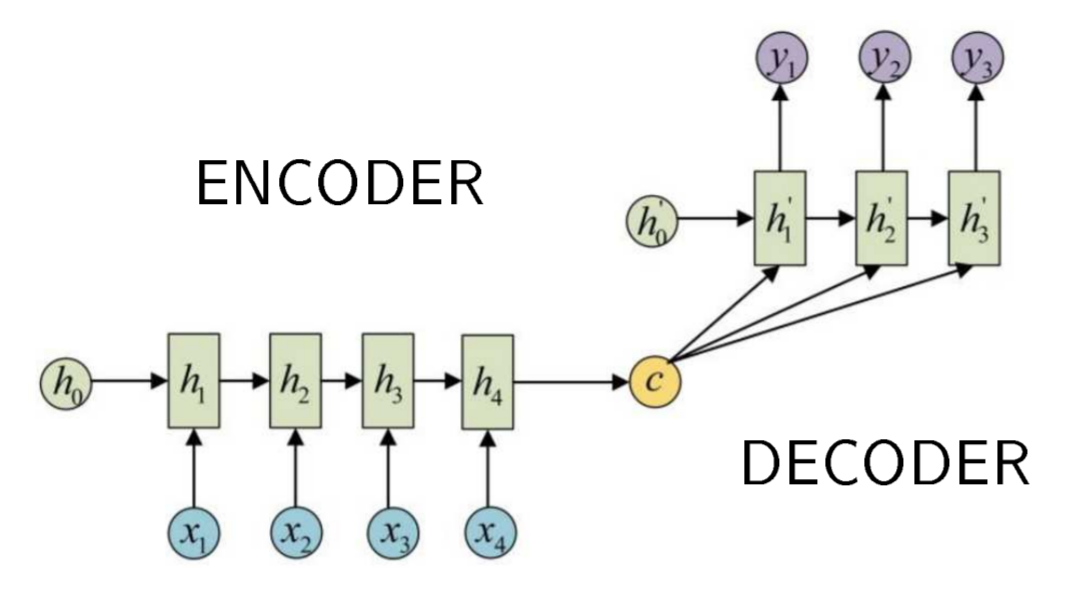
\includegraphics[keepaspectratio,
                    width=.5\paperwidth]{seq2seq.png}
   \end{center}

  \begin{center}
    \begin{align*}
      h_i &= f_{in}(x_i, h_{i-1}) \\
      {\color{red}h_t^\prime} &{\color{red}= f_{out}(h_{t-1}^\prime,y_{t-1},c)} \\
      y_t &= f_{y}(h_t^\prime, y_{t-1})
    \end{align*}
  \end{center}
\end{frame}


\begin{frame}
  \frametitle{Summary}
\begin{itemize}
    \item Recurrent neural networks — a simple, powerful and flexible approach to solving various machine learning problems
    \item Vanilla RNNs are simple, but still not good enough
    \item So you need to use LSTM or GRU, and seq2seq architecture
    \item LSTM prevents zeroing gradients 
    \item Clipping helps with <<explosion of gradients>>
    \item We need deeper understanding, both theoretical and practical — there are many open questions
  \end{itemize}
  \pause
  What else can you see?
  \begin{itemize}
    \item \href{https://www.youtube.com/watch?v=iX5V1WpxxkY}{Lecture 10} of the course <<CS231n>> by Andrej Karpathy at Stanford
    \item How to \href{http://karpathy.github.io/2019/04/25/recipe/}{train neural networks}?
    \item \href{https://github.com/yandexdataschool/Practical_DL/tree/fall21/week06_rnn}{Similar lecture} of the School of Data Analysis course (in Russian)
    \item \href{https://www.youtube.com/watch?v=_JuQcodHANs}{Fresh interview} of Andrej Karpathy by Lex Fridman
  \end{itemize}
\end{frame}

\end{document}
